\chapter{GUI application}

This milestone covers the development effort for implementing stage \ref{num:stage9} described in \Nameref{sec:developmentStages}.

\section{AvaloniaUI}

As decided in the project planning milestone (see chapter \ref{chap:evalProjPlan}), \textit{AvaloniaUI} will be used as the \ref{itm:gui} framework.
Because \textit{AvaloniaUI} uses \ref{itm:xaml} for defining the \ref{itm:ui} and utilizes \ref{itm:mvvm} as its architectural pattern \cite{katz_mvvm_2022}, it was not too difficult to use it thanks to previous experience with \ref{itm:wpf} (one of Microsoft's official \ref{itm:gui} frameworks).

The only drawback of the framework is that it still needs a stable release. That entails the unreliability of the framework and the possibility of breaking changes. For example, \textit{AvaloniaUI} version 0.10.15 broke \ref{itm:ui} components for displaying images. Nevertheless, it is backed up by a passionate community of developers that ensure a quick resolution of any discovered issues.

The open-source community added significant value to the framework by developing additional libraries such as \textit{AvaloniaBehaviors}, or \textit{FluentAvaloniaUI}, both of used by ModularDoc. The former extends missing features for manipulating the \ref{itm:ui} based on defined triggers. The latter provides the \textit{Fluent} theme for \textit{AvaloniaUI}. \textit{Fluent} is Microsoft's modern design system that can be seen utilized across all of its applications \cite{microsoft_microsoft_nodate}. By default, the \textit{AvaloniaUI} uses an outdated version of \textit{Fluent} and, in some cases, does not respect the design system. So, the \textit{FluentAvaloniaUI} library is essential for having a modern, good-looking design.

\section{Decoupling via MVVM}

\textit{AvaloniaUI} is a beautiful \ref{itm:gui} framework; however, it is not a first-party Microsoft product - this poses a higher risk of project abandonment. Moreover, users of the ModularDoc might not like \textit{AvaloniaUI} and wish to have the tool hosted online in an \ref{gloss:aspnetcore} web application. Doubling down on a highly configurable tool results in an application with its business logic utterly independent from the \ref{itm:ui} framework
That is achieved using \ref{itm:mvvm} in combination with a \ref{itm:di} framework like \textit{Autofac}.

\ref{itm:mvvm} (Model, View, View Model) allows natural decoupling of the \ref{itm:ui} (View), from the business logic (View Model) and data (Model) \cite{katz_mvvm_2022}. However, \ref{itm:mvvm} alone still introduces some coupling of the \ref{itm:ui} to the host application, as it must still reference the specific views for, e.g., navigation. Such references are decoupled by abstracting each view with its interface representation. The specific views would then be provided via \textit{Autofac}. This allows easy swapping of views either based on \textit{AvaloniaUI} or some other framework.

To take it a step further, the view models are also be abstracted in the same way and provided via \textit{Autofac}. In this case, the benefit is higher application testability, as abstracted view models can be mocked.

\section{Application structure}

The \ref{itm:gui} application serves only as a configuration creator and executor for the available plugins.
Thus, the application requires minimum work on the \ref{itm:ui} side and will consist of the following pages:
\begin{itemize}
    \item Home page.
    \item Settings page.
    \item About page.
    \item Configuration wizard.
    \item Summary page.
\end{itemize}

Each page was mocked to understand the application's \ref{itm:ui} layout before its implementation.

\subsection{Home page}

The home page presents the user with the available plugins. The \ref{itm:ux} is simple, as the user should only select the desired plugin, see its description, and decide whether they wish to use it or cancel.
Additionally, the user may wish to load a previously created configuration, so an option for loading configurations is available.
Finally, the user can search for the desired plugin via the search filter if the application has many of them.

\begin{figure}[H]
    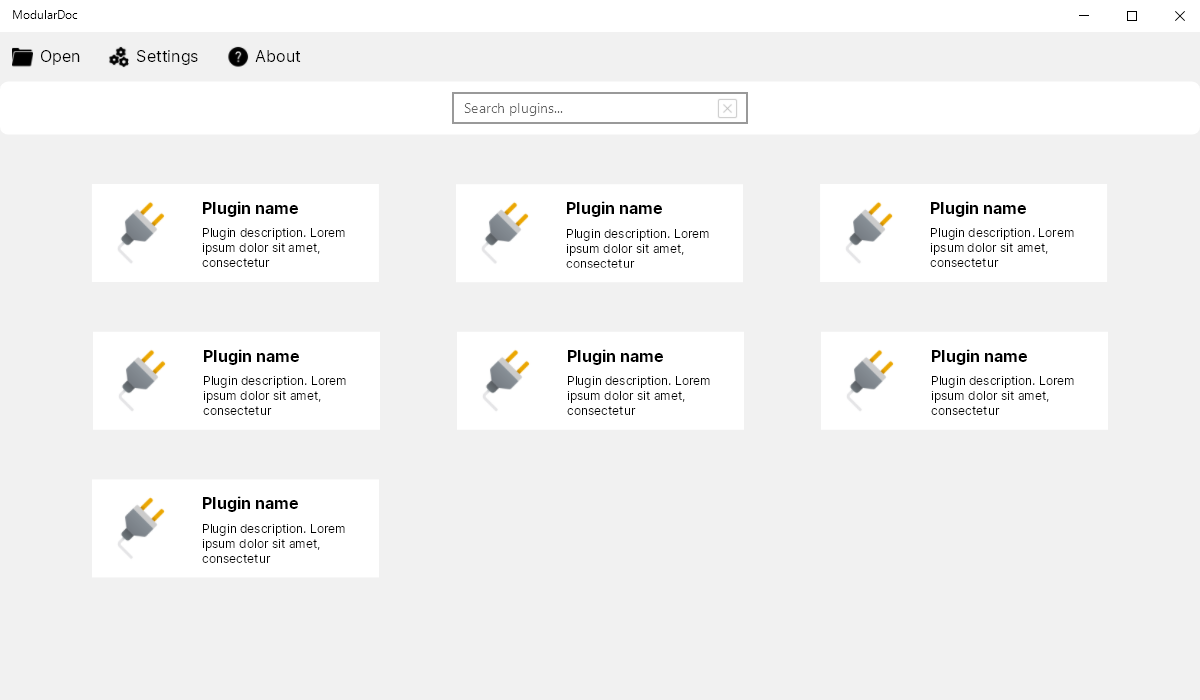
\includegraphics[width=\linewidth]{img/mockHome.png}
    \label{fig:homePage}
    \caption{Mock of the home page}
\end{figure}

\begin{figure}[H]
    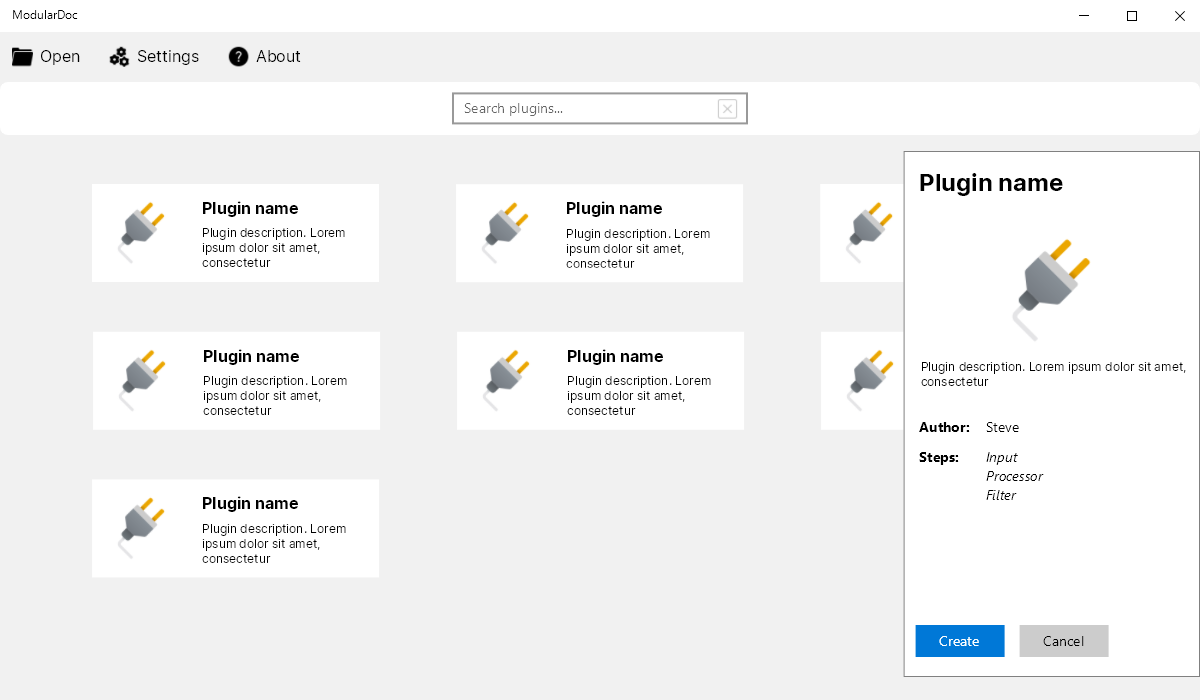
\includegraphics[width=\linewidth]{img/mockHome-PluginSelected.png}
    \label{fig:homePagePluginSelected}
    \caption{Mock of the home page with a plugin selected}
\end{figure}

\pagebreak
\subsection{Settings page}

The settings page allows the user to configure the application. Since adding multicultural support would add more complexity to the project, the only setting provided on this page is a toggle between the light and dark mode themes. Any settings added in the future will be present on this page.

\begin{figure}[H]
    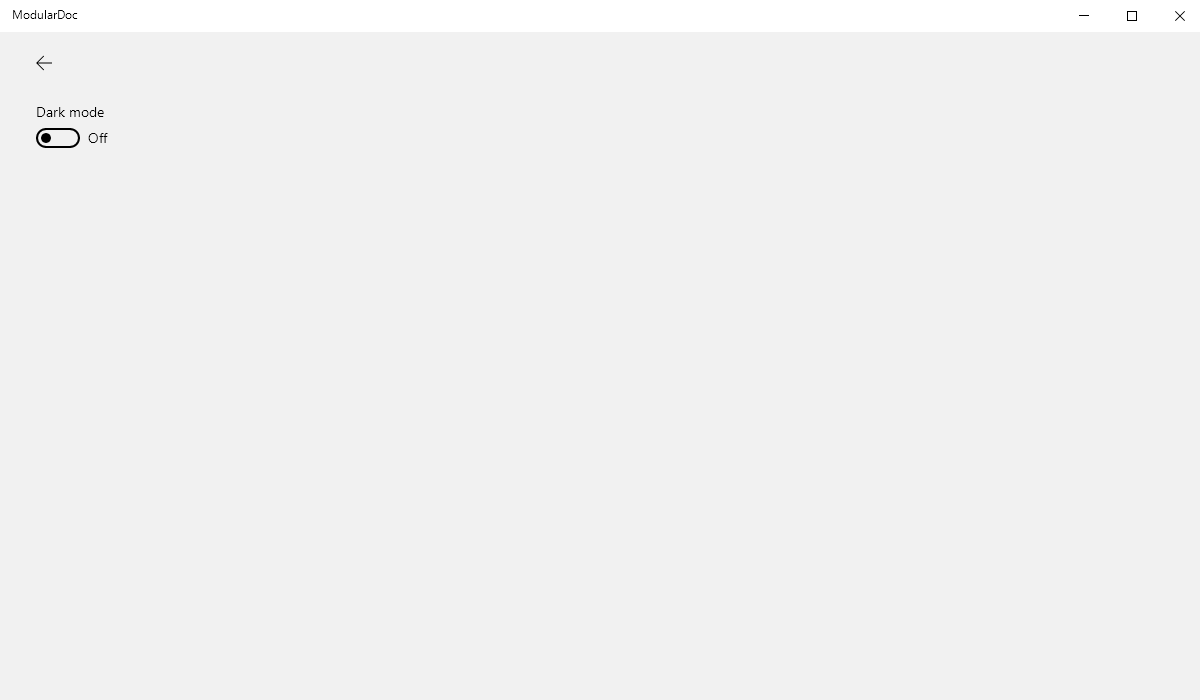
\includegraphics[width=\linewidth]{img/mockSettings.png}
    \label{fig:settingsPage}
    \caption{Mock of settings page}
\end{figure}

\subsection{About page}

The about page would present the user with necessary information about the application, references to used libraries, and possibly usage instructions. However, the content of this page was neither designed nor prepared. That is because it had a low priority; thus, it was excluded from this development phase.

\pagebreak
\subsection{Configuration wizard}

The configuration wizard is responsible for displaying configuration steps provided by the selected plugin. The plugin provides the \ref{itm:ui} of each step; thus, this page's design is only concerned with correctly displaying the steps and controls for navigating between them.

The user can proceed to the next step only if the current one is configured correctly.

\begin{figure}[H]
    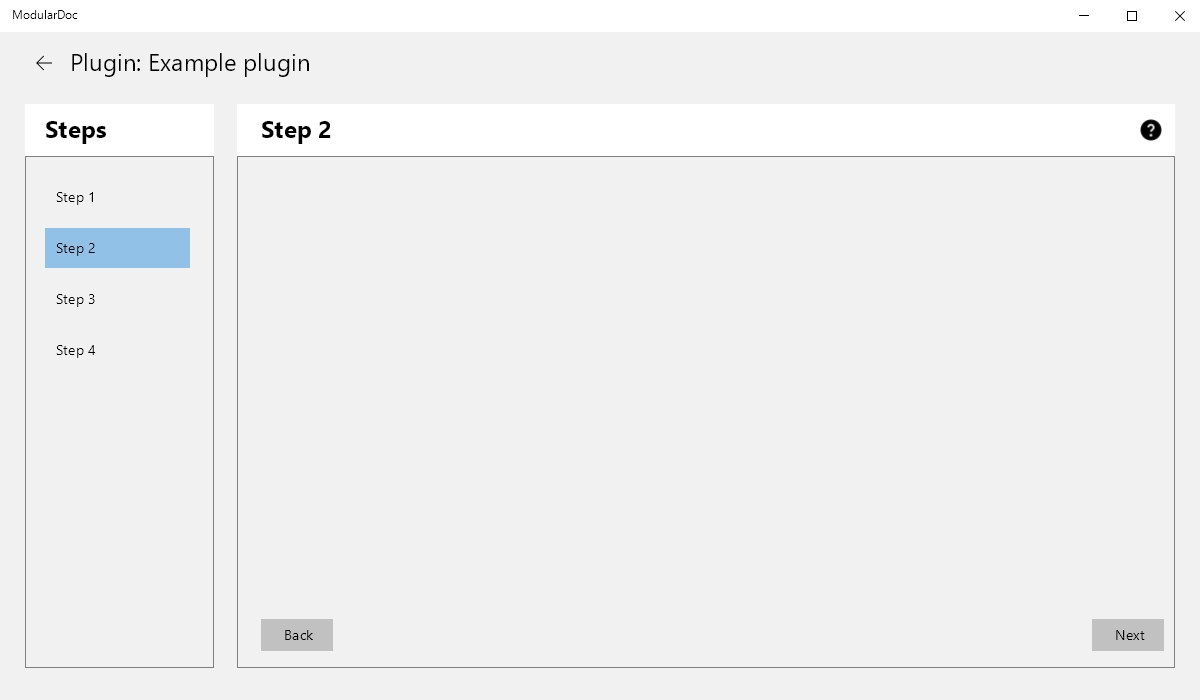
\includegraphics[width=\linewidth]{img/mockConfigurator.png}
    \label{fig:configuratorPage}
    \caption{Mock of configuration wizard}
\end{figure}

\pagebreak
\subsection{Summary page}

The summary is responsible for executing the selected plugin's configuration after loading it or configuring it for the first time. In addition, it displays the progress of each plugin step and logs what each process is doing.

At this stage, the user can save the created configuration and return either to the first configuration step or to the home page without saving.

\begin{figure}[H]
    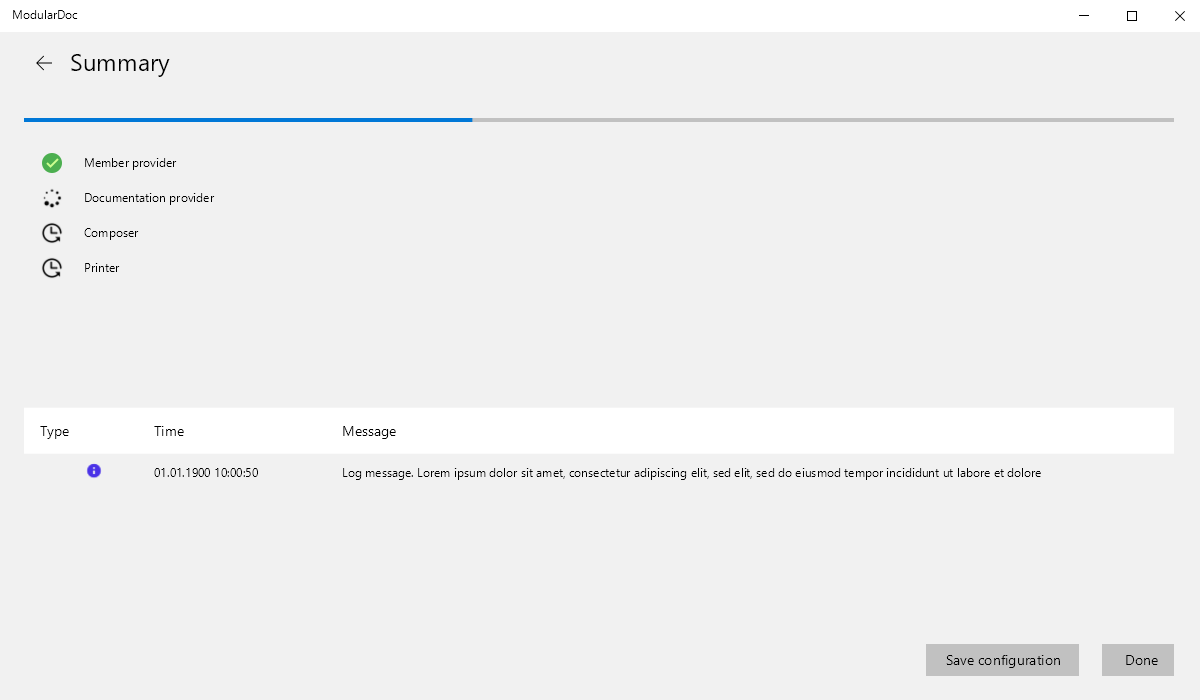
\includegraphics[width=\linewidth]{img/mockSummary.png}
    \label{fig:summaryPage}
    \caption{Mock of summary page}
\end{figure}